\section*{Mise en place de la topologie} 
\vspace{0.3cm}

\subsection{Confirmation de la configuration en utilisant ping}
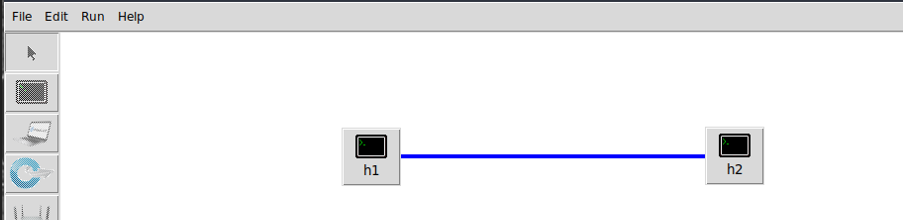
\includegraphics[width=1\textwidth]{./images/topology.png} \\
\subsubsection{Changement du masque de sous-réseau}
\vspace{0.3cm}
Initialement, le masque de sous-réseau était défini à /8, ce qui signifie que les 8 premiers bits de l'adresse IP représentaient la partie réseau, et les 24 bits restants étaient réservés pour les hôtes.
Cependant, on doit modifier ce masque de sous-réseau de /8 à /16. Cela signifie que les 16 premiers bits définissent désormais la partie réseau de l’adresse IP, tandis que les 16 bits restants sont utilisés pour les hôtes.\\

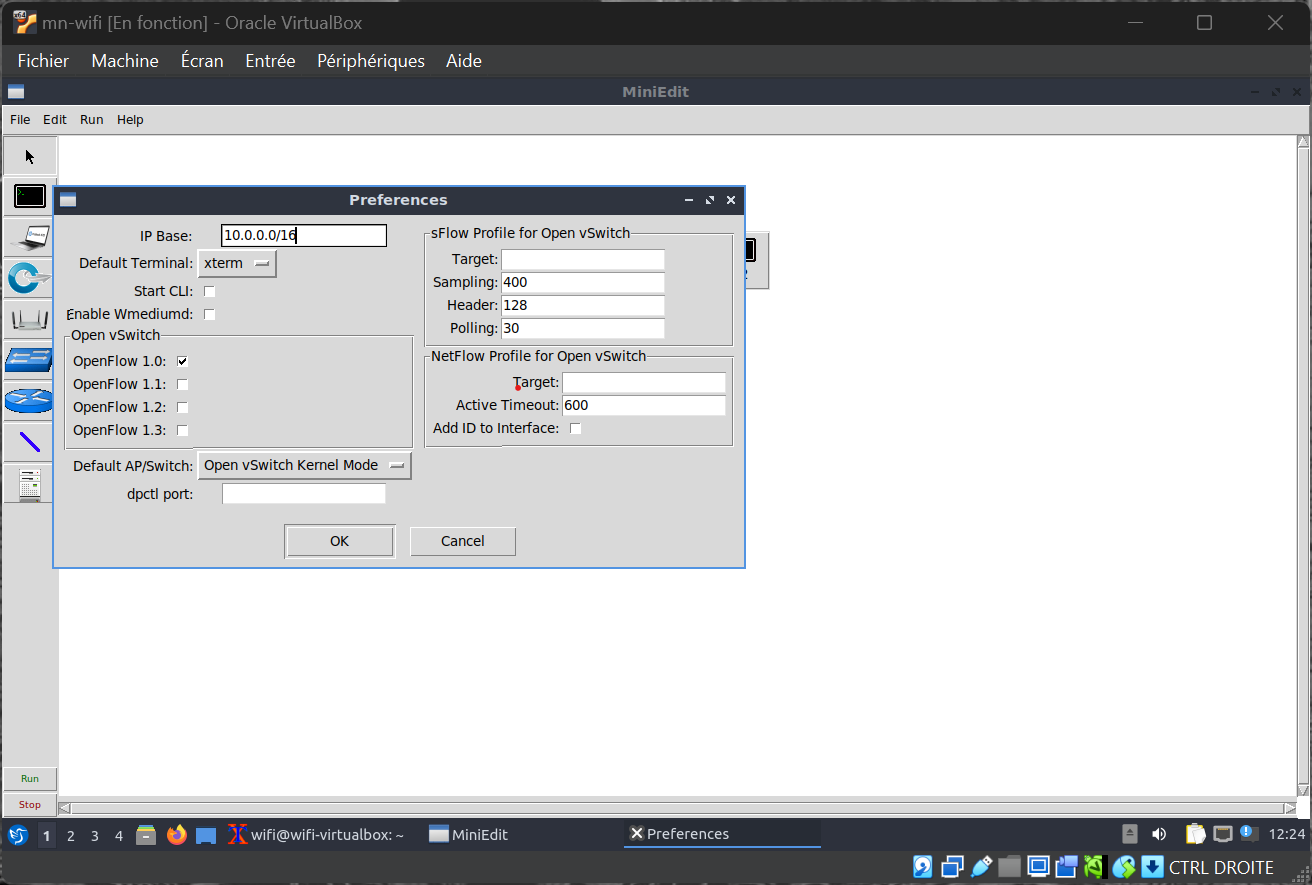
\includegraphics[width=1\textwidth]{./images/IpBaseSetup.png} \\


\subsubsection{Attribution des Adresses IP aux Hôtes}
\begin{itemize}
    \item h1 : 10.25.0.26
    \item h2 : 10.25.0.27
\end{itemize}


\subsubsection{Ping}
Lorsque la commande ping est lancée, h2 envoie un paquet ICMP Echo Request à l'adresse IP de h1. Ce paquet contient 64 bytes de données par défaut, ainsi qu'un numéro de séquence pour suivre les paquets envoyés (icmp\_seq).

h1 reçoit ce paquet ICMP Echo Request et le traite. En réponse, il génère un paquet ICMP Echo Reply, qui contient les mêmes données que celles envoyées par h2.

Ce paquet Echo Reply est renvoyé à l'appareil source (h2). Lorsque h2 reçoit la réponse, il mesure le temps que le paquet a mis pour faire l'aller-retour, appelé Round Trip Time (RTT).

Le terminal affiche ainsi le TTL (Time to Live), qui mesure le nombre de routeurs ou de sauts traversés par le paquet avant d'atteindre sa destination.

\begin{itemize}
    \item \textbf{64 bytes} : La taille du paquet ICMP envoyé et reçu (64 octets par défaut).
    \item \textbf{from 10.25.0.26} : L'adresse IP de la machine qui a répondu à la requête ICMP (ici, h1).
    \item \textbf{icmp\_seq=i} : Le numéro de séquence du paquet envoyé, permettant de vérifier l'ordre et la réception des paquets.
    \item \textbf{ttl=64} : Le Time to Live du paquet, qui est initialement défini par l'appareil source est décrémenté de 1 à chaque routeur traversé.
    \item \textbf{time=0.072 ms} : Le temps que le paquet a mis pour faire l’aller-retour, en millisecondes, indiquant la latence ou délai entre les deux appareils.
\end{itemize}
\begin{center}
    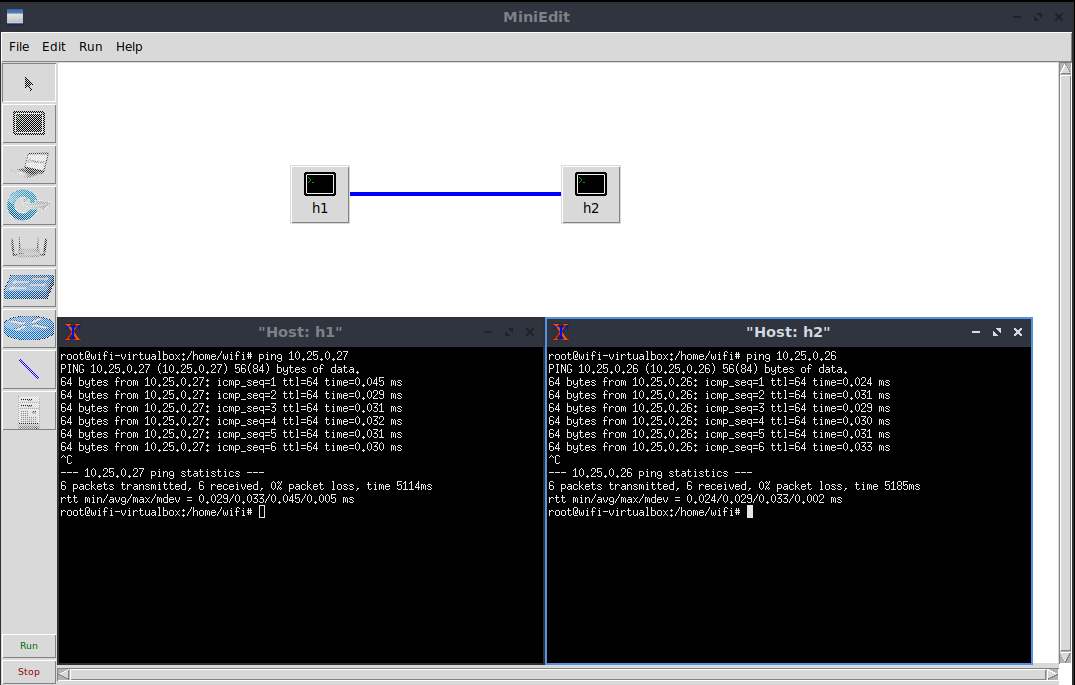
\includegraphics[width=1\textwidth]{./images/TopologiePing.png}
\end{center}

\subsection{Tests}
\subsubsection{T1.1 : Varier le débit du lien entre H1 et H2 ( mettre la même valeur sur les deux machines ).}
\vspace{0.5cm}
\hspace{0.5cm}\textbf{1:} `ip link show` et `tc qdisc show dev h1-eth0`
\begin{center}
    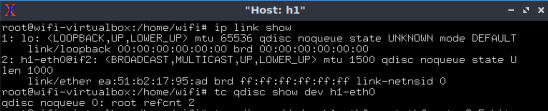
\includegraphics[width=1\textwidth]{./images/ShowDefaultQdisc.png}
\end{center}
Le résultat de ip link show indiquera si l'interface h1-eth0 est active et prête à envoyer des données, tandis que le résultat de tc qdisc show montrera les règles en place pour le contrôle du trafic, y compris les limites de bande passante et la gestion de la latence. 

\vspace{1cm}

\textbf{2:} `tc qdisc add dev h1-eth0 root handle 1:0 tbf rate 2.5gbit burst 32kbit latency 400ms (resp h2-eth0)`
\begin{center}
    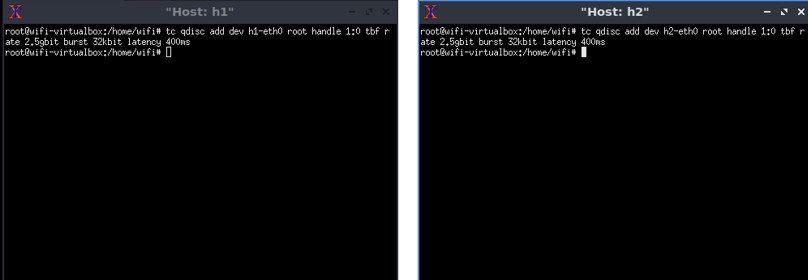
\includegraphics[width=1\textwidth]{./images/1smaller.png}
\end{center}
Les deux interfaces h1-eth0 et h2-eth0 sont configurées pour limiter le débit à 2,5 Gbps.(E1)

\vspace{1cm}
\textbf{3:} `iperf3 -s pour h1 , iperf3 -c ip-h1`
\begin{center}
    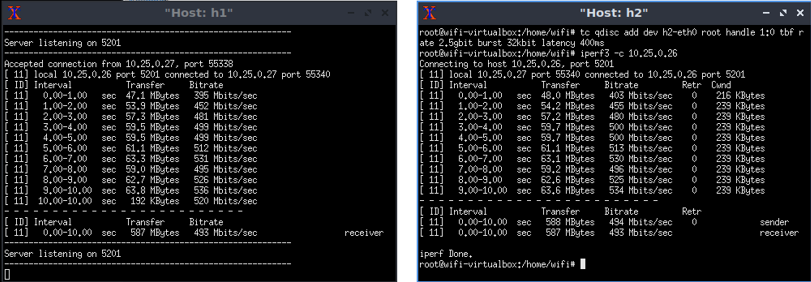
\includegraphics[width=1\textwidth]{./images/2smaller.png}
\end{center}
Pour h1 : iperf3 -s lance iperf3 en mode serveur , elle accepte la connexion au client h2\\
pour h2 : iperf3 -c 10.25.0.26 lance iperf3 en mode client et connecte au seurveur h1
\\
\\Les débits moyens de 493 Mbits/sec et 494 Mbits/sec sont observés respectivement pour le serveur et le client. Cela montre que les deux hôtes peuvent échanger des données à une vitesse proche de 500 Mbits/sec.
\\
\\Bien que les commandes tc qdisc add initiales aient fixé un débit maximum de 2,5 Gbits/sec, les résultats montrent des débits bien inférieurs à cette limite (environ 493-494 Mbits/sec).
\\ 
\\les memes tests sont fait pour une valeur moyenne (DL * 0.05) et une valeur élevée (DL par defaut), on preésente les captures : 

\vspace{1cm}
\textbf{4:} `tc qdisc add dev h1-eth0 root handle 1:0 tbf rate 125Mbit burst 32kbit latency 400ms (resp h2-eth0)`
\begin{center}
    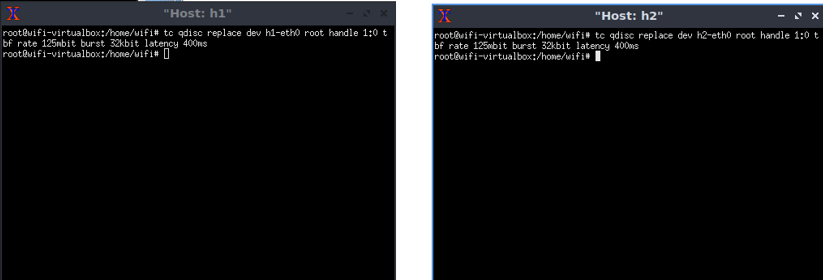
\includegraphics[width=1\textwidth]{./images/ValuerMoyenneCommande.png} \\
    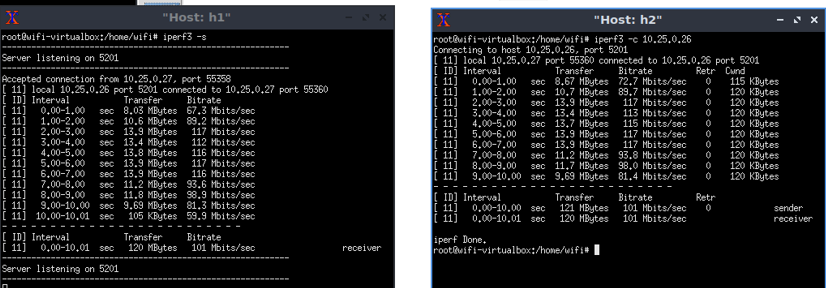
\includegraphics[width=1\textwidth]{./images/ValeurMoyenneResultat.png}
\end{center}
\vspace{1cm}
\hspace{0.5cm}\textbf{5:} `tc qdisc add dev h1-eth0 root handle 1:0 tbf rate 625Mbit burst 32kbit latency 400ms (resp h2-eth0)`
\begin{center}
    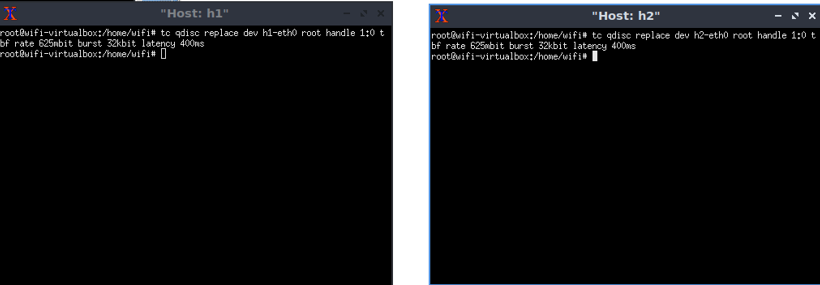
\includegraphics[width=1\textwidth]{./images/ValuerDefautCommande.png} 
    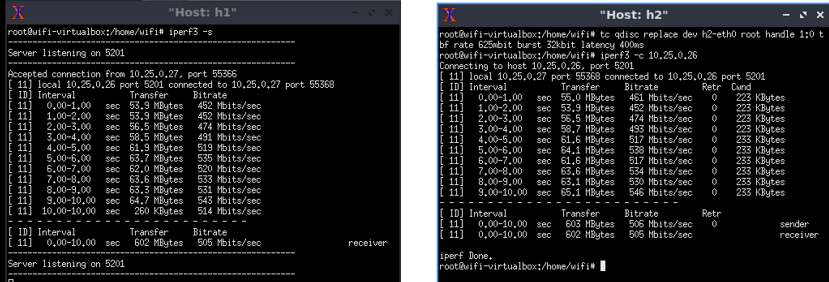
\includegraphics[width=1\textwidth]{./images/ValuerDefautResultat.png}
\end{center}
\textbf{Courbe T1.1:} 

Le graphe montre une relation entre le débit physique du lien (DL) et le débit applicatif mesuré lors des tests entre les machines h1 et h2.
\\
\\Le débit applicatif augmente de manière significative avec le débit physique , puis se stabilise, indiquant que d'autres facteurs, comme les limites du CPU ou l'outil iperf3 lui meme, empêchent une augmentation proportionnelle, malgré l'augmentation du débit physique.
 
\subsubsection{T1.2 : Fixer la valeurdu débit sur le lien entre H1 et le Switch à 1Gb/s et varier le débit sur H2.}
\vspace{0.5cm}
\begin{center}
    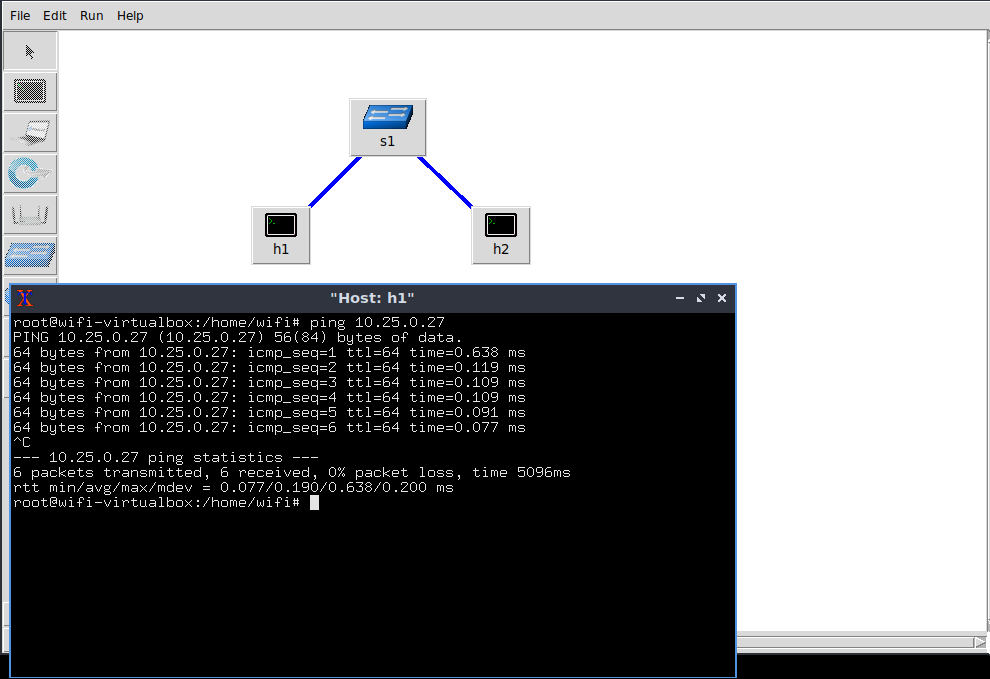
\includegraphics[width=1\textwidth]{./images/T1.2TopologyAndPing.png}
\end{center}
\textbf{1:} `tc qdisc add dev h2-eth0 root netem rate 125mbit`
\begin{center}
    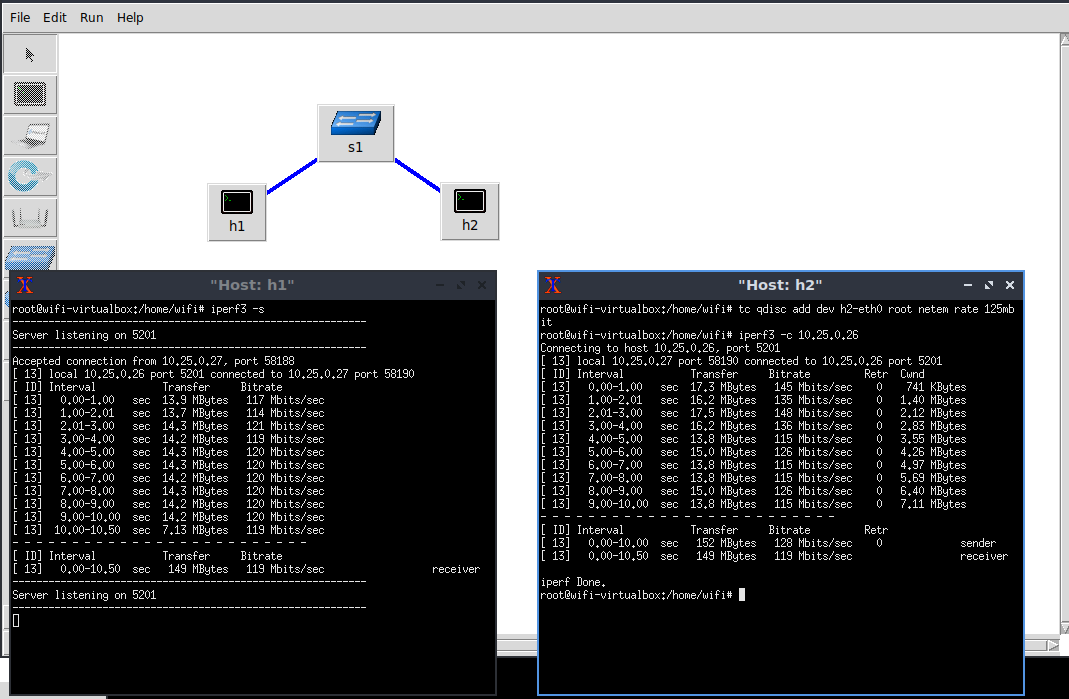
\includegraphics[width=1\textwidth]{./images/T1.2/125test2.png}
    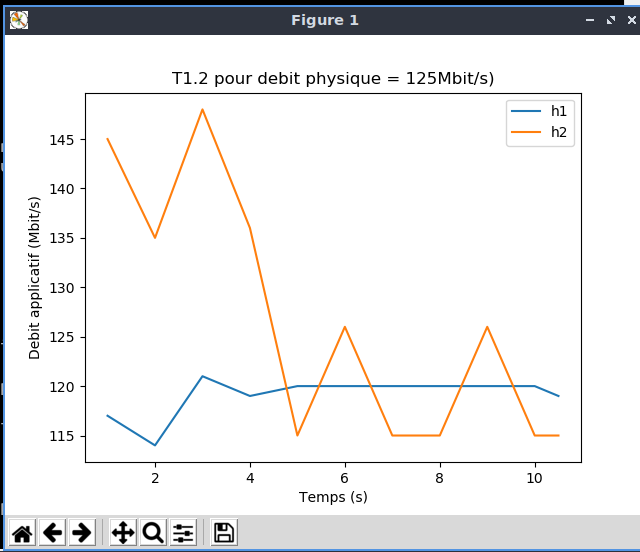
\includegraphics[width=1\textwidth]{./images/T1.2/courbe125test2.png}
    
\end{center}
\textbf{Observation :}\\
Débit de H1 (ligne bleue) : Le débit applicatif mesuré sur h1 reste relativement stable, oscillant entre 115 Mbit/s et 125 Mbit/s tout au long du test. Même si le lien physique entre H1 et le switch est de 1 Gbit/s, le débit observé n’atteint jamais cette valeur maximale théorique.

Débit de H2 (ligne orange) : Le débit applicatif de H2 fluctue considérablement, atteignant parfois des pics autour de 145 Mbit/s, mais chutant aussi à des valeurs proches de 120 Mbit/s ou même légèrement en dessous.
\vspace{1cm}
\\
\textbf{Explications :} 
\\
Bien que la liaison entre h1 et le switch soit fixée à 1 Gbit/s, c'est le lien entre H2 et le switch qui impose une limite plus contraignante de 125 Mbit/s.\\
Dans ce type de configuration, le débit total du transfert est dicté par le maillon le plus faible de la chaîne, en l’occurrence la connexion limitée entre H2 et le switch. Le lien de 1 Gbit/s entre h1 et le switch ne peut donc pas être exploité pleinement tant que H2 ne peut pas recevoir ou envoyer des données plus rapidement que 125 Mbit/s.\\
\\
L'outil iperf3 utilise généralement le protocole TCP, qui ajuste automatiquement le débit en fonction des capacités du réseau. TCP surveille les capacités des deux hôtes et ajuste son débit en fonction des retours qu’il reçoit (accusés de réception des paquets).
Ici, TCP détecte que le débit sur le lien entre H2 et le switch est limité à 125 Mbit/s et ajuste donc la transmission des données pour s’adapter à cette contrainte, expliquant pourquoi le débit de h1 reste autour de 115 à 125 Mbit/s.
Le protocole TCP est conçu pour éviter la surcharge du réseau et s’adapte dynamiquement aux conditions de congestion, ce qui pourrait aussi expliquer pourquoi le débit de H2 est plus instable, car le lien est proche de sa capacité maximale.\\
\\
\textbf{2:} `tc qdisc add dev h2-eth0 root netem rate 625mbit `
\begin{center}
    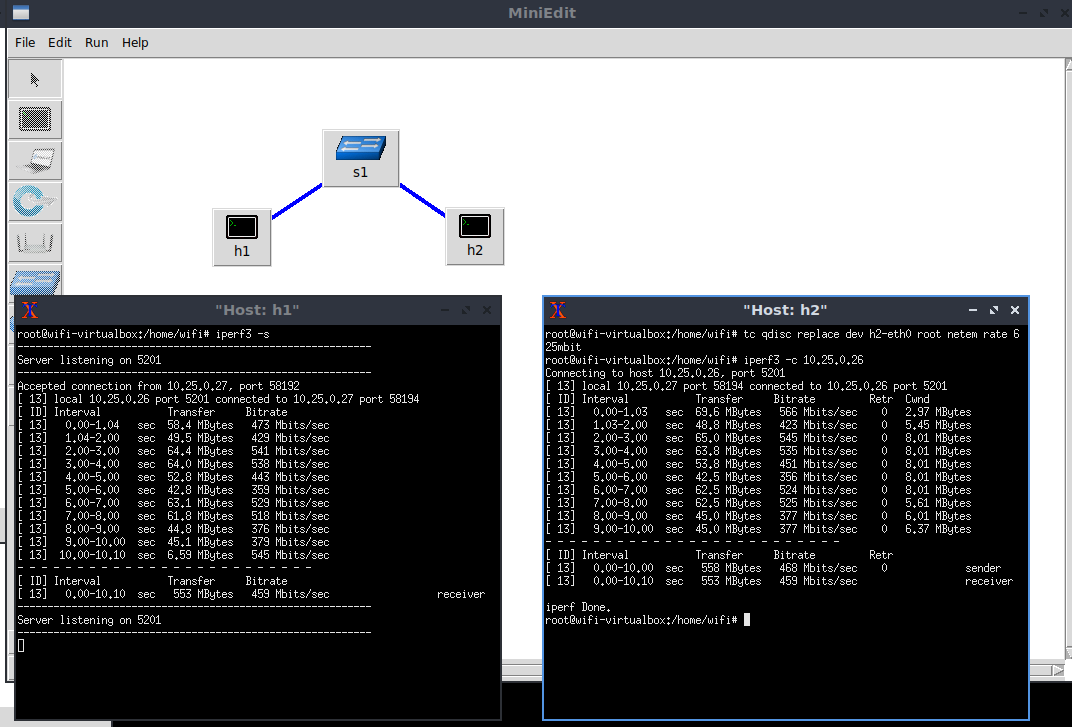
\includegraphics[width=1\textwidth]{./images/T1.2/625test2.png}
    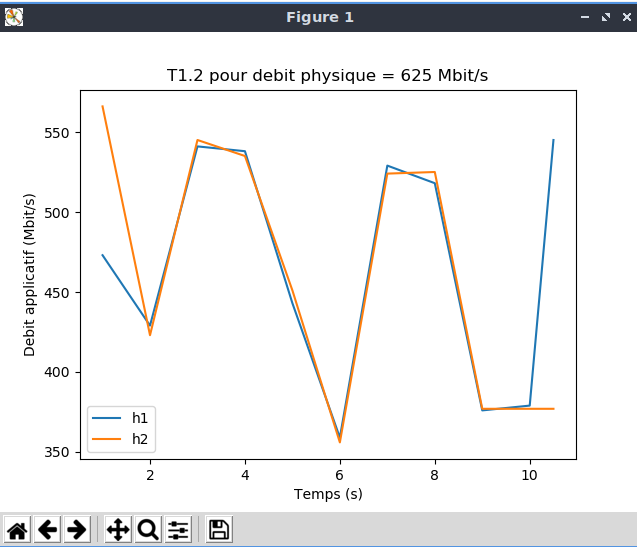
\includegraphics[width=1\textwidth]{./images/T1.2/courbe625test2.png}
\end{center}
\textbf{Observation :}\\
Débit de h1 (ligne bleue) : Le débit applicatif mesuré sur h1 varie entre 350 Mbit/s et environ 550 Mbit/s.
Débit de h2 (ligne orange) : Le débit applicatif sur H2 suit une courbe similaire à celle de h1.
\\
\textbf{Explication} :\\
Le fait que les deux débits (h1 et h2) suivent un schéma similaire de montée et descente suggère que la limitation du débit physique à 625 Mbit/s entre H2 et le switch influence directement les deux hôtes. Comme le débit de H2 est limité par le lien physique, le switch agit comme un point de congestion, entraînant des fluctuations du débit applicatif.
\vspace{1cm}
\\
\textbf{3:} `tc qdisc add dev h2-eth0 root netem rate 2.5gbit`
\begin{center}
    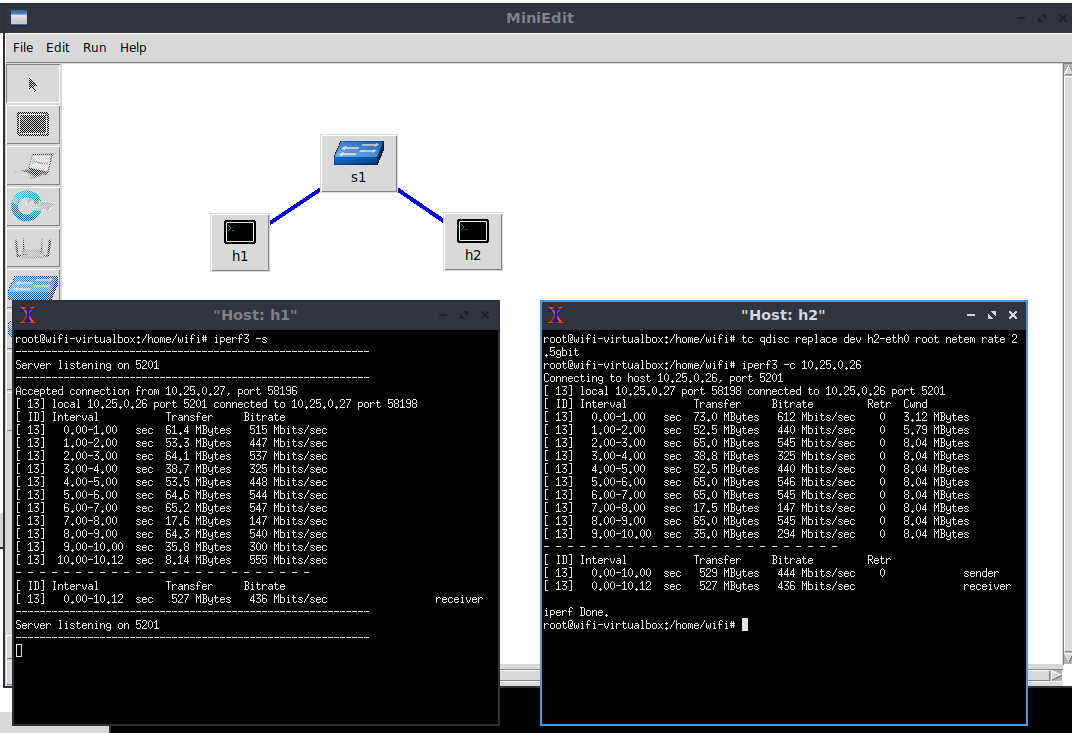
\includegraphics[width=1\textwidth]{./images/T1.2/2500test2.png}
    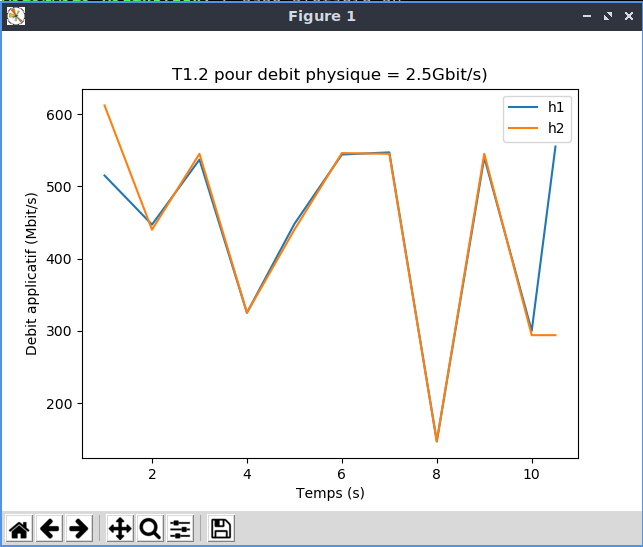
\includegraphics[width=1\textwidth]{./images/T1.2/courbe2500test2.png}
\end{center}

\newpage
\textbf{Courbe T1.2:} 




